%%%%%%%%%%%%%%%%%%%%%%%%%%%%%%%%%%%%%%%%%
% Beamer Presentation
% LaTeX Template
% Version 1.0 (10/11/12)
%
% This template has been downloaded from:
% http://www.LaTeXTemplates.com
%
% License:
% CC BY-NC-SA 3.0 (http://creativecommons.org/licenses/by-nc-sa/3.0/)
%
%%%%%%%%%%%%%%%%%%%%%%%%%%%%%%%%%%%%%%%%%

%----------------------------------------------------------------------------------------
%	PACKAGES AND THEMES
%----------------------------------------------------------------------------------------

\documentclass{beamer}

\mode<presentation> {

% The Beamer class comes with a number of default slide themes
% which change the colors and layouts of slides. Below this is a list
% of all the themes, uncomment each in turn to see what they look like.

%\usetheme{default}
%\usetheme{AnnArbor}
%\usetheme{Antibes}
%\usetheme{Bergen}
%\usetheme{Berkeley}
%\usetheme{Berlin}
%\usetheme{Boadilla}
%\usetheme{CambridgeUS}
%\usetheme{Copenhagen}
%\usetheme{Darmstadt}
%\usetheme{Dresden}
%\usetheme{Frankfurt}
%\usetheme{Goettingen}
%\usetheme{Hannover}
%\usetheme{Ilmenau}
%\usetheme{JuanLesPins}
%\usetheme{Luebeck}
\usetheme{Madrid}
%\usetheme{Malmoe}
%\usetheme{Marburg}
%\usetheme{Montpellier}
%\usetheme{PaloAlto}
%\usetheme{Pittsburgh}
%\usetheme{Rochester}
%\usetheme{Singapore}
%\usetheme{Szeged}
%\usetheme{Warsaw}

%\bibliographystyle{abbrvnat}
\bibliographystyle{plain} % reference type change : [1] , [2] , ... (+ usepackage(natbib))
% As well as themes, the Beamer class has a number of color themes
% for any slide theme. Uncomment each of these in turn to see how it
% changes the colors of your current slide theme.

%\usecolortheme{albatross}
%\usecolortheme{beaver}
%\usecolortheme{beetle}
%\usecolortheme{crane}
%\usecolortheme{dolphin}
%\usecolortheme{dove}
%\usecolortheme{fly}
%\usecolortheme{lily}
%\usecolortheme{orchid}
%\usecolortheme{rose}
%\usecolortheme{seagull}
%\usecolortheme{seahorse}
%\usecolortheme{whale}
%\usecolortheme{wolverine}

%\setbeamertemplate{footline} % To remove the footer line in all slides uncomment this line
\setbeamertemplate{footline}[page number] % To replace the footer line in all slides with a simple slide count uncomment this line

\setbeamertemplate{navigation symbols}{} % To remove the navigation symbols from the bottom of all slides uncomment this line
}
\setbeamertemplate{caption}[numbered]{} % figure number attached : figure 1 , 2 ,...
\usepackage{natbib} % reference type change : [1] , [2] , ... 
\usepackage{graphicx} % Allows including images
\graphicspath{{./img/}}
\usepackage{caption}
\usepackage[normalem]{ulem} % cancel line. when you input the ulem.sty in your file package will work on.
\usepackage{subcaption}
\usepackage{booktabs} % Allows the use of \toprule, \midrule and \bottomrule in tables
\usepackage{amsmath}
\usepackage{amssymb}
\usepackage{amsthm}
%\usepackage {tikz}
\usepackage{tkz-graph}
\usepackage {xcolor}
\definecolor {processblue}{cmyk}{0.96,0,0,0}

%----------------------------------------------------------------------------------------
%	TITLE PAGE
%----------------------------------------------------------------------------------------

\title[Short title]{0. Review }

\author{Dong-Gyu, Lee}
\institute[] % Your institution as it will appear on the bottom of every slide, may be shorthand to save space
{
	Dept. of Statistics, KU% Your institution for the title page
\medskip
}
\date{2020, Apr 3} % Date, can be changed to a custom date

\begin{document}

\begin{frame}
\titlepage % Print the title page as the first slide
\end{frame}

\begin{frame}{Contents}
\frametitle{Contents}
	\tableofcontents 
\end{frame}

%----------------------------------------------------------------------------------------
%	PRESENTATION SLIDES
%----------------------------------------------------------------------------------------
\section{Analysis Goal}
\begin{frame}{Today's Goal}
	\begin{itemize}
		\item Before studying the Jupiter code for AlexNet, VGG, GoogleNet, and ResNet, let's review the core of each model.
	\end{itemize}
\end{frame}


\section{ILSVRC}
\begin{frame}{ILSVRC}
	\begin{itemize}
		\item ImageNet Large Scale Visual Recognition Challenge(ILSVRC) was an annual computer vision contest held between 2010 and 2017.
		\item It's also called ImageNet Challenge.
	\end{itemize}
	\vspace{10pt}
	\begin{figure}[h]		
		\centering
		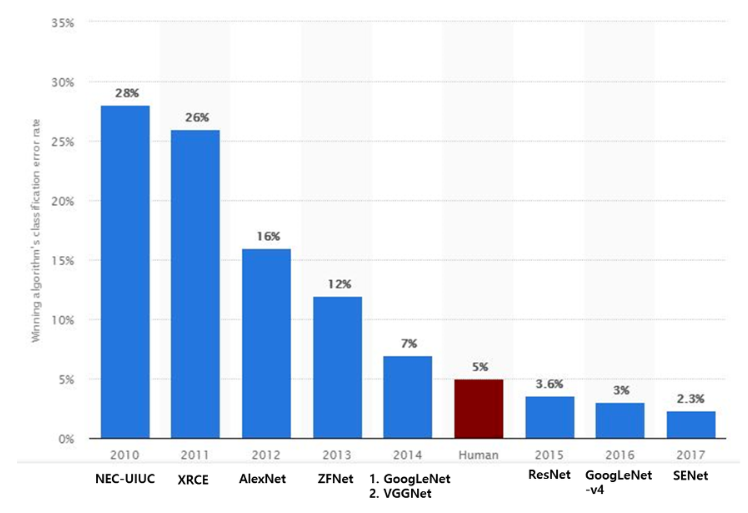
\includegraphics[scale=0.4]{./ilsvrc/ILSVRC.PNG}
		\caption{ILSVRC(Classification)}
		\label{ilsvrc}
	\end{figure}
\end{frame}


\begin{frame}{ILSVRC}
	\begin{itemize}
		\item For this challenge, the training data is a subset of ImageNet: 1000 synsets, 1.2 million images.
		\item There are 50K images for validation and 150K images for testing.
	\end{itemize}
	\vspace{10pt}
	\begin{figure}[h]		
		\centering
		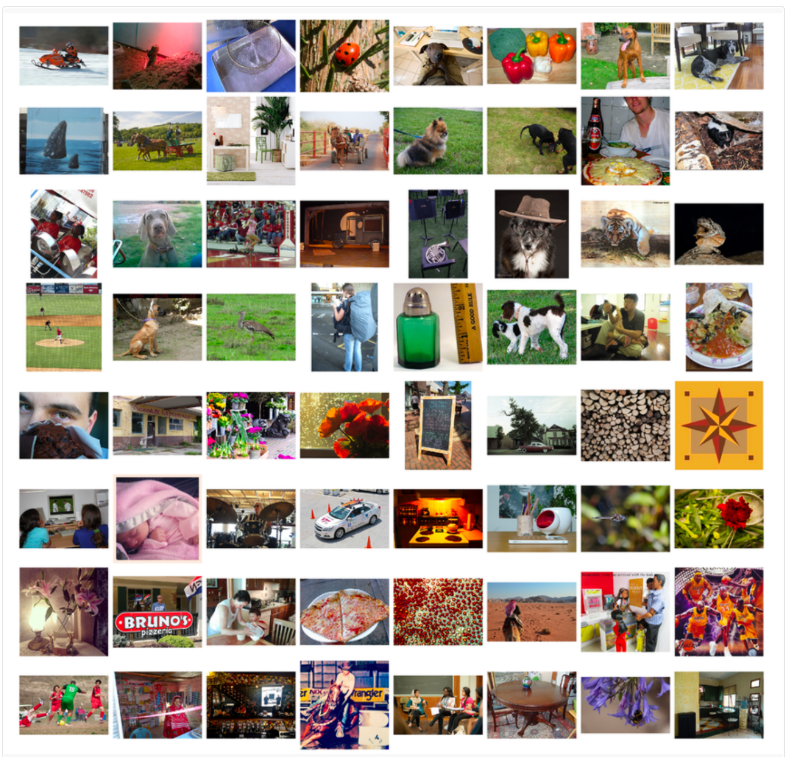
\includegraphics[scale=0.35]{./ilsvrc/ilsvrc_2.PNG}
		\caption{ImageNet Dataset Used in the ILSVRC}
		\label{ilsvrc:images}
	\end{figure}
\end{frame}


\section{FER2013}
\begin{frame}{FER2013}
	\begin{itemize}
		\item FER2013 dataset consists of 35,887 grayscale, 48x48 sized face images with various emotions - 7 emotions.
		\item Emotion labels in the dataset(imbalanced) : Angry, Disgust, Fear, Happy, Sad, Surprise, Neutral
	\end{itemize}
	\vspace{10pt}
	\begin{figure}[h]		
		\centering
		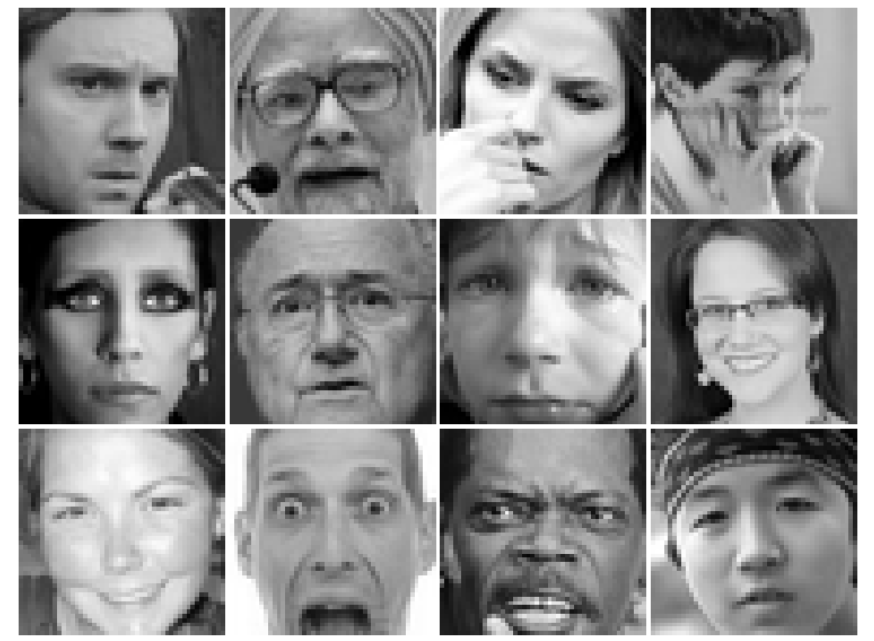
\includegraphics[scale=0.22]{./fer/FER2013.PNG}
		\caption{FER2013 Dataset}
		\label{ilsvrc:images}
	\end{figure}
	\begin{itemize}
		\item However, in FER2013 dataset, quite a few images are incorrectly labeled.
		\item So the FER Plus dataset was newly created in 2016.
	\end{itemize}
\end{frame}


\section{AlexNet}
\begin{frame}{1. AlexNet}
	\vspace{10pt}
	\begin{itemize}
		\item The number of parameters of AlexNet\cite{alexnet} is almost 62 million.
	\end{itemize}
	\vspace{10pt}
	\begin{figure}[h]		
		\centering
		{\includegraphics[page={1},width=0.47\textwidth]{./alex/Alexnet_1.PNG}}
		\quad
		{\includegraphics[page={2},width=0.47\textwidth]{./alex/AlexNet_2.PNG}}
		\caption{AlexNet}
		\label{Alexnet}
	\end{figure}
\end{frame}


\begin{frame}{1. AlexNet}
	\begin{itemize}
		\item Tanh vs ReLU.
		\item Dropout.
		\item Overlapping pooling.
		\item LRN.
		\item Data augmentation.
	\end{itemize}
	\begin{figure}[h]		
		\centering
		\subfloat[ReLU]
		{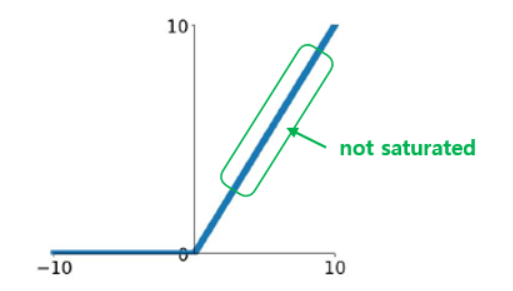
\includegraphics[page={1},width=0.5\textwidth]{./alex/ReLU.PNG}}
		\quad
		\subfloat[Dropout]
		{\includegraphics[page={2},width=0.35\textwidth]{./alex/dropout.PNG}}
		\caption{AlexNet Characteristic}
		\label{alexnet:char}
	\end{figure}
\end{frame}


\section{VGG}
\begin{frame}{2. VGG}
	\vspace{10pt}
	\begin{itemize}
		\item The number of parameters of VGG16\cite{vgg} is almost 138 million.
	\end{itemize}
	\vspace{10pt}
	\begin{figure}[h]		
		\centering
		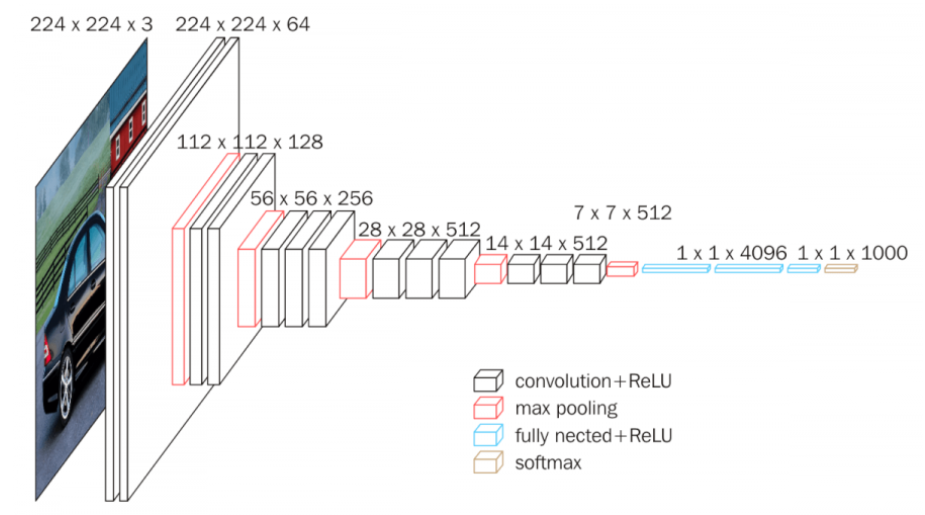
\includegraphics[scale=0.5]{./vgg/VGG_2.PNG}
		\caption{VGG16 Structure}
		\label{VGG16}
	\end{figure}
\end{frame}


\begin{frame}{2. VGG}
	\begin{itemize}
		\item Interested in deeper layers.
		\item Only 3x3 convolution.
		\item VGG11, VGG13, VGG16, VGG19.
	\end{itemize}
	\begin{figure}[h]		
		\centering
		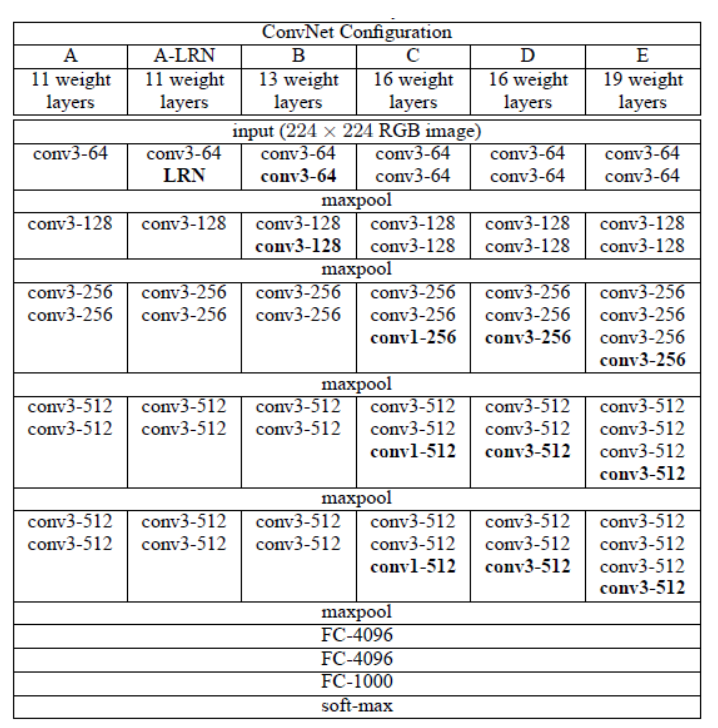
\includegraphics[scale=0.38]{./vgg/VGG_1.PNG}
		\caption{VGG}
		\label{VGG}
	\end{figure}
\end{frame}


\section{GoogLeNet}
\begin{frame}{3. GoogLeNet}
	\vspace{10pt}
	\begin{itemize}
		\item The number of parameters of GoogLeNet\cite{googlenet} is almost 5 million.
	\end{itemize}
	\vspace{10pt}
	\begin{figure}[h]		
		\centering
		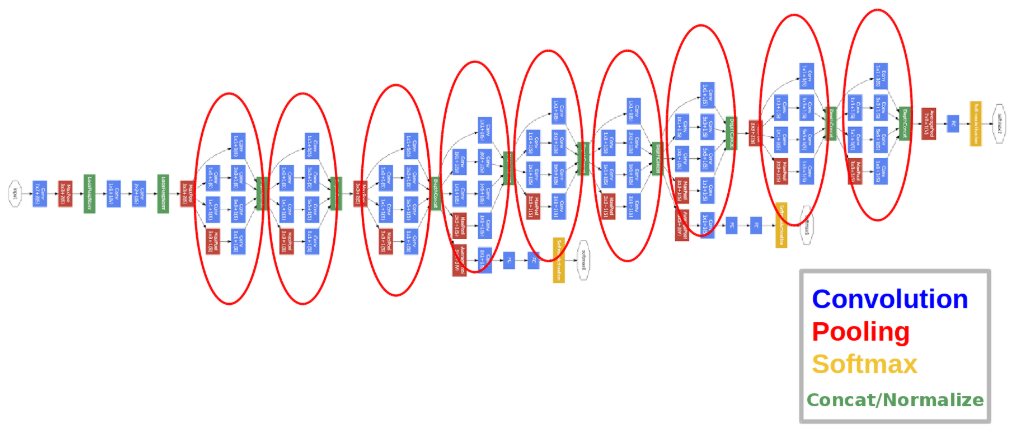
\includegraphics[scale=0.5]{./google/googlenet.PNG}
		\caption{GoogLeNet Structure}
		\label{GoogLeNetstr}
	\end{figure}
\end{frame}


\begin{frame}{3. GoogLeNet}
	\begin{itemize}
		\item 22 layers.
		\item Inspired by network in network(NIN)\cite{nin}.
		\item Inception module(sparse \& dense connectivity, 1x1 convolution).
		\item Auxiliary classifier(0.3:0.3:1).
		\item Global Average Pooling(GAP).
	\end{itemize}
	\vspace{10pt}
	\begin{figure}[h]		
		\centering
		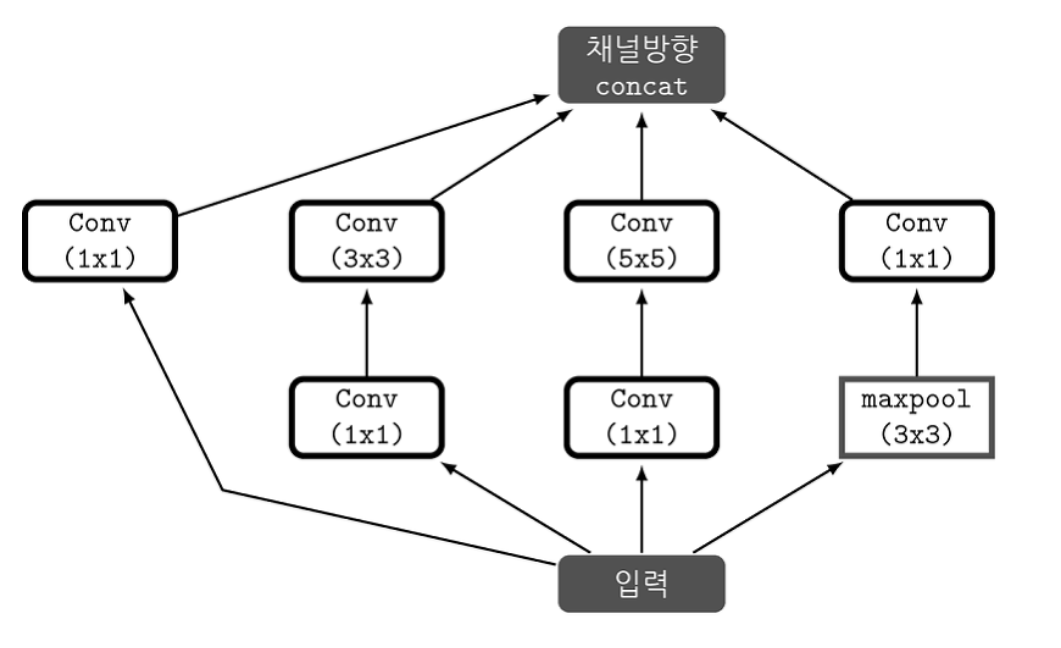
\includegraphics[scale=0.32]{./google/inception_module.PNG}
		\caption{Inception Module}
		\label{inception}
	\end{figure}
\end{frame}


\begin{frame}{3. GoogLeNet}
	\vspace{10pt}
	\begin{itemize}
		\item Ref) Network in Network :
	\end{itemize}
	\vspace{10pt}
	\begin{figure}[h]		
		\centering
		\subfloat[Linear Convolution Layer]
		{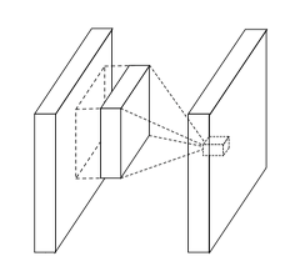
\includegraphics[page={1},width=0.4\textwidth]{./google/nin1.PNG}}
		\quad
		\subfloat[Mlpconv Layer]
		{\includegraphics[page={2},width=0.4\textwidth]{./google/nin2.PNG}}
		\label{nin}
	\end{figure}
\end{frame}


\begin{frame}{3. GoogLeNet}
	\vspace{10pt}
	\begin{itemize}
		\item GoogLeNet Summary :
	\end{itemize}
	\vspace{10pt}
	\begin{figure}[h]		
		\centering
		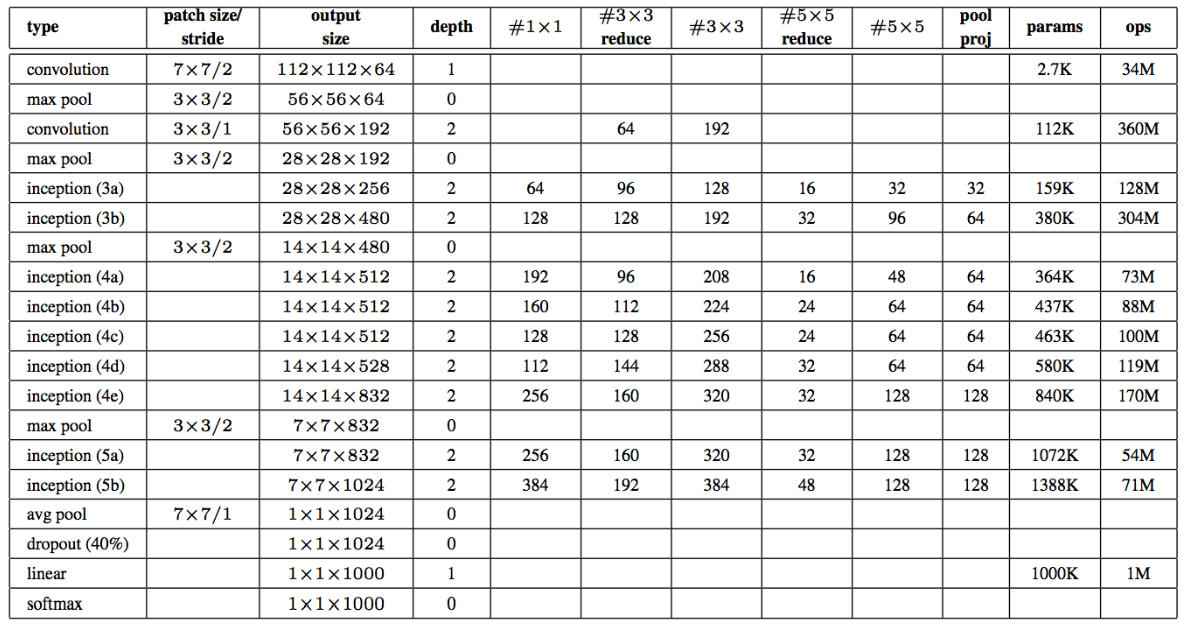
\includegraphics[scale=0.4]{./google/googlenet_3.PNG}
		\caption{GoogLeNet}
		\label{googlenet}
	\end{figure}
\end{frame}


\section{ResNet}
\begin{frame}{4. ResNet}
	\vspace{10pt}
	\begin{itemize}
		\item 18,34,50,101,152 layers.
		\item The number of parameters of ResNet34\cite{resnet},\cite{resnetbn} is almost 21 million.
	\end{itemize}
	\vspace{10pt}
	\begin{figure}[h]		
		\centering
		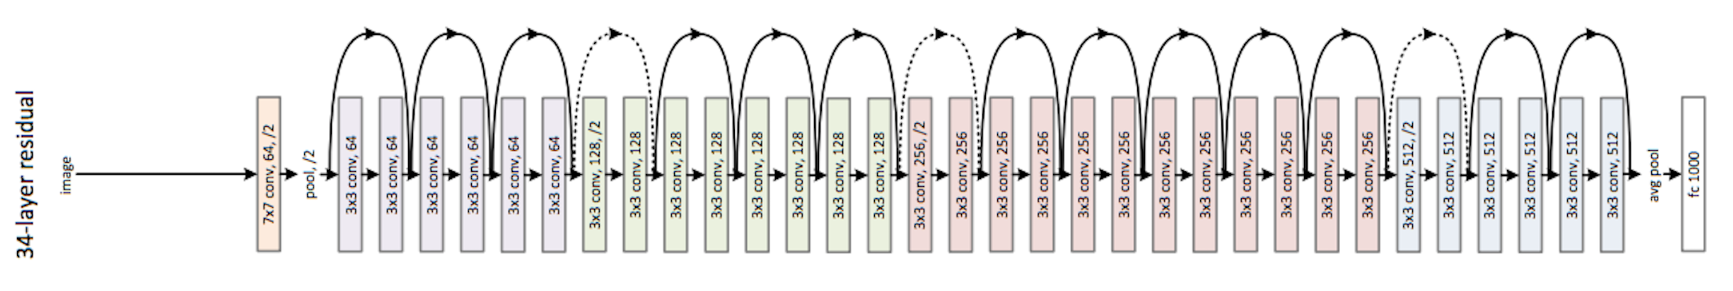
\includegraphics[scale=0.3]{./res/resnet34.PNG}
		\caption{ResNet34 Structure}
		\label{resnet34}
	\end{figure}
\end{frame}


\begin{frame}{4. ResNet}
	\begin{itemize}
		\item Degradation.
		\item Residual learning.
		\item Skip(Shortcut) connection.
		\item Bottleneck architecture.
		\item Batch Normalization\cite{bn}.
	\end{itemize}
	\vspace{5pt}
	\begin{figure}[h]		
		\centering
		\subfloat[Training]
		{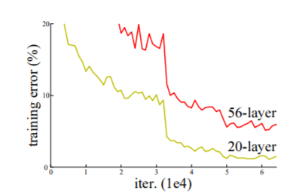
\includegraphics[page={1},width=0.4\textwidth]{./res/degrad_train.PNG}}
		\quad
		\subfloat[Test]
		{\includegraphics[page={2},width=0.4\textwidth]{./res/degrad_test.PNG}}
		\caption{Degradation Problem}
		\label{degradation}
	\end{figure}
\end{frame}


\begin{frame}{4. ResNet}
	\vspace{10pt}
	\begin{itemize}
		\item Residual Learning :
	\end{itemize}
	\begin{figure}[h]		
		\centering
		\subfloat[Simple Neural Network]
		{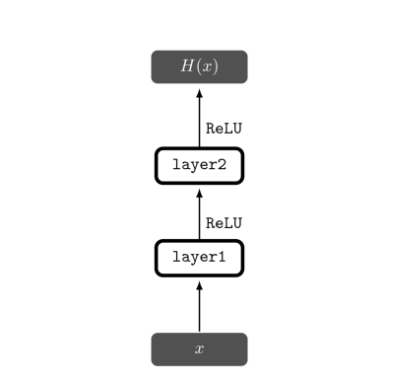
\includegraphics[page={1},width=0.45\textwidth]{./res/normal.PNG}}
		\quad
		\subfloat[Skip Connection in ResNet]
		{\includegraphics[page={2},width=0.45\textwidth]{./res/learning.PNG}}
		\caption{Residual Learning}
		\label{residuallearning}
	\end{figure}
\end{frame}


\begin{frame}{4. ResNet}
	\vspace{10pt}
	\begin{itemize}
		\item Bottleneck Architecture :
	\end{itemize}
	\vspace{10pt}
	\begin{figure}[h]		
		\centering
		\subfloat[Block for ResNet-18/34]
		{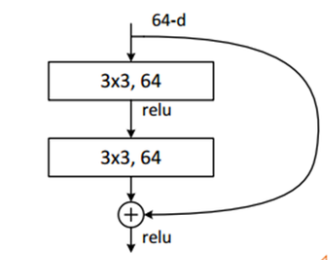
\includegraphics[page={1},width=0.4\textwidth]{./res/resblock1.PNG}}
		\quad
		\subfloat[Block for ResNet-50/101/152]
		{\includegraphics[page={2},width=0.4\textwidth]{./res/resblock2.PNG}}
		\caption{Right: Bottlneck Architecture}
		\label{resblock}
	\end{figure}
\end{frame}


\begin{frame}{4. ResNet}
	\vspace{10pt}
	\begin{itemize}
		\item ResNet Summary :
	\end{itemize}
	\vspace{10pt}
	\begin{figure}[h]		
		\centering
		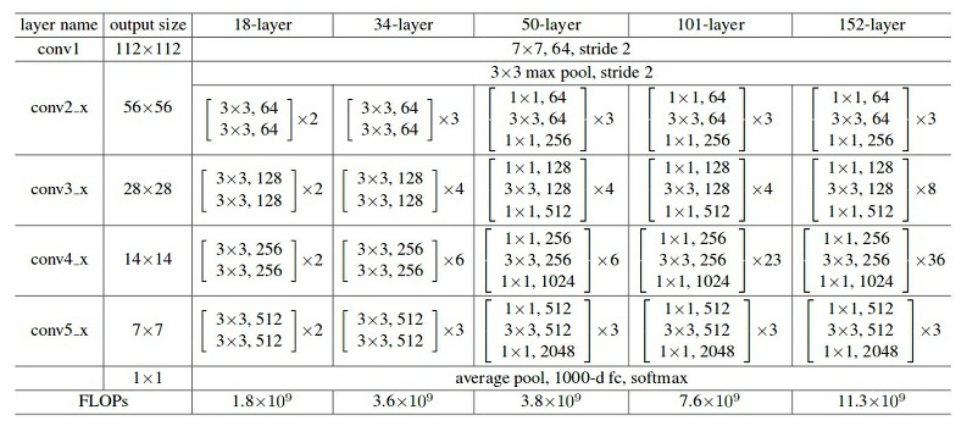
\includegraphics[scale=0.55]{./res/resnetstr.PNG}
		\caption{ResNet}
		\label{resnet}
	\end{figure}
\end{frame}


\begin{frame}{4. ResNet}
	\vspace{10pt}
	\begin{itemize}
		\item ResNet Result :
	\end{itemize}
	\vspace{10pt}
	\begin{figure}[h]		
		\centering
		\subfloat[Before]
		{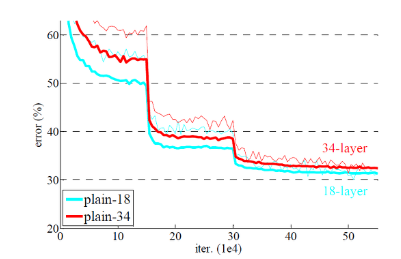
\includegraphics[page={1},width=0.45\textwidth]{./res/resnet1834_1.PNG}}
		\quad
		\subfloat[After]
		{\includegraphics[page={2},width=0.45\textwidth]{./res/resnet1834_2.PNG}}
		\caption{ResNet Effect}
		\label{effect}
	\end{figure}
\end{frame}


\section{Reference}
\begin{frame}[allowframebreaks]{Reference}
	\bibliography{references}
\end{frame}

\end{document}
